%========= Introduction
\section{Introduction}~\label{sec:introduction}
{O}{ne}-third of music streaming on smartphones is intended to influence affective states (such as uplifting motivation during mundane tasks or to purge negative emotions) \cite{wadley2019use}. According to a recent survey by a group of researchers in Spain, 73.8\% of respondents reported using online music as a means of managing their emotions \cite{martin2021music}. Using social media applications was the most effective technique to self-regulate mood during the COVID-19 pandemic \cite{prikhidko2020effect}, \cite{shao2021social}, \cite{colasante2020any}. Pre-pandemic, a different survey found that 87\% of teens and adults would go online for ways to deal with stress, anxiety, or depression, but just 20\% of them would consider seeking professional help \cite{rideout2018digital}. Some instances of emotions driving smartphone usage in daily life include listening to music while exercising, watching online videos during daily commutes, scrolling through social media while waiting in a queue, and browsing shopping websites at the workplace.
    
\begin{figure}[h]
  
    \centering
    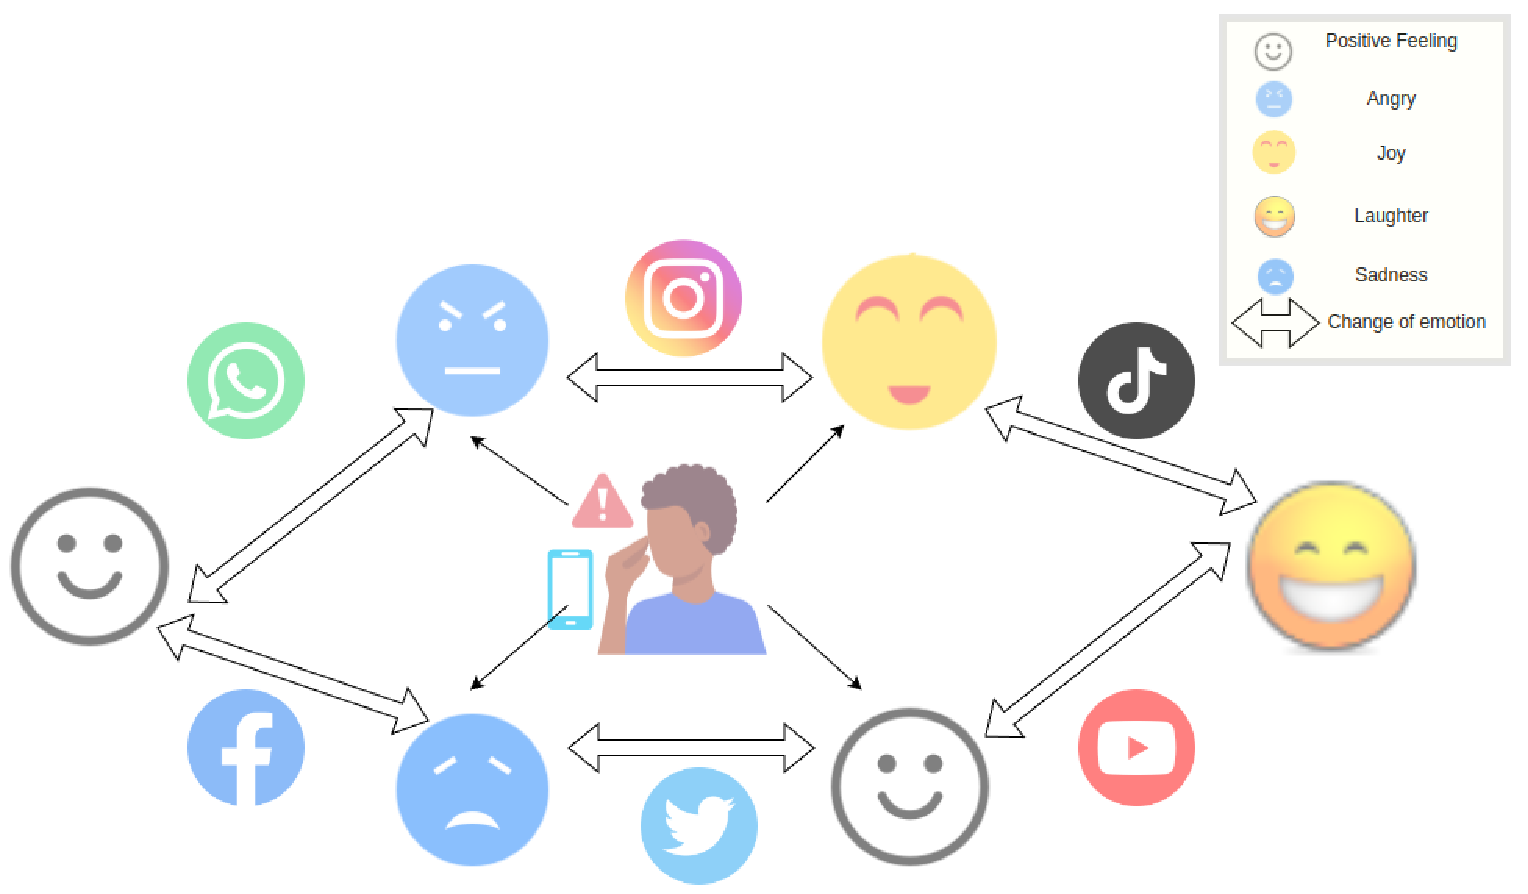
\includegraphics[width=10cm,height=10cm,keepaspectratio]{DER.pdf}
  \caption{Digital Emotion Regulation using Social Media}
  \label{fig:SMER}
  \end{figure}
The practice of consciously modifying one's affective state is called emotion regulation (ER) \cite{gross1998emerging}. The ability to successfully perform emotion regulation is essential to function effectively in everyday life, to act appropriately in everyday interactions, or merely for hedonic purposes \cite{webb2012dealing}. The ubiquity of digital technology has produced a plethora of prospects for understanding, managing and influencing the world we live in. Digital technology is now being used judiciously to influence our affective states (such as emotions, mood, and stress levels), a process known as digital emotion regulation (DER). In addition to its novelty and scope, understanding digital emotion regulation can facilitate the advancement of the ethical design, development, and application of technology \cite{wadley2020digital}.


The rise in popularity of social media applications has led to significant virtualisation of the day-to-day activities in our lives. Since these applications provide a variety of dimensions for expression and consumption, traditional forms of engagement, leisure and amusement have also been revolutionised by this digitalisation \cite{schull2012addiction}. The COVID-19 pandemic made it difficult to socialise offline, thus more people than ever are choosing to spend their social lives online. Emotions are intertwined in our daily affairs and shape our interactions because they form an essential component of human behaviour influencing how we think and act. Our experiences elicit emotional responses, and these emotions frame our actions \cite{gross1998emerging}, \cite{gross2015emotion}. The same is also true for digital technology and social media. It has been observed that emotional states impact interactions with technology, such as joystick movements, typing errors, as well as typing speed. Recent studies have established a correlation between emotional states and the number of application launches, duration of application use, and type of application used, demonstrating that there is a bidirectional relationship between emotions and social media use \cite{sarsenbayeva2020does}. People seem to have created a toolkit that allows them to actively appropriate and integrate a variety of applications to manage emotions in everyday life \cite{smith2022digital}. Scrolling through social media for distraction, watching cat videos for stress relief, texting a friend for support, following an inspirational person to focus on success, and sharing emotions through status updates are a few examples of DER via digital media platforms as shown in Figure-\ref{fig:SMER}. The omnipresence of social media applications has optimised our ability to regulate emotions at any time or place by allowing us to fine-tune our strategies for specific situations and engage in emotion regulation more frequently.

\subsection{Background and Motivation}
Emotion regulation is a goal-oriented process in which people monitor, evaluate, and change their emotional responses to achieve their objectives. This process is dynamic in nature, which means it involves a continuous series of adaptive behaviours and responses. It can happen explicitly or implicitly \cite{braunstein2017explicit}, \cite{gyurak2011explicit}.
Understanding emotion regulation necessitates learning about the emotion regulation process as well as the motivation for doing so. By classifying emotion regulation strategies into five categories according to where they appear in the sequence of emotion generation, Gross's process model describes how emotion regulation is performed. \cite{wadley2020digital}, \cite{gross1998emerging}. Situation selection is the first intervention, which entails going into situations that might evoke desired emotions or staying away from scenarios that might induce undesirable emotions. Situation modification makes it possible to control emotions by altering specific aspects of a situation directly after it has been encountered and before an emotional reaction has formed completely. This is accomplished by shifting one's focus from or toward emotion-relevant features deliberately, or by reevaluating a situation to change the way of its emotional impact through cognitive change. Lastly, response modulation can be used to change the physiological, behavioural, or experiential components of an emotional response even after it has already occurred (e.g., exhibiting intensified facial expressions).  Figure-\ref{fig:Process} describes the process of emotion regulation and the strategies a social media user may employ to modify their affective state. Tamir's motive taxonomy, which divides the goal of emotion regulation into two categories, hedonic and instrumental, with additional classifications, may be used to explain emotion regulation motivations \cite{wadley2020digital}, \cite{tamir2016people}. Hedonic motives (Prohedonic and Contrahedonic) entail engaging in emotion regulation in order to experience or avoid certain emotions; typically, pleasant emotions are enhanced while painful emotions are diminished. Instrumental motives (Performance, Epistemic, and Social) are motivations that people have when they think that a particular affective state could help accomplish a task, meet a performance target, or demonstrate appropriate expressions and behaviours \cite{wadley2020digital}.
\begin{figure}[h]
  
    \centering
    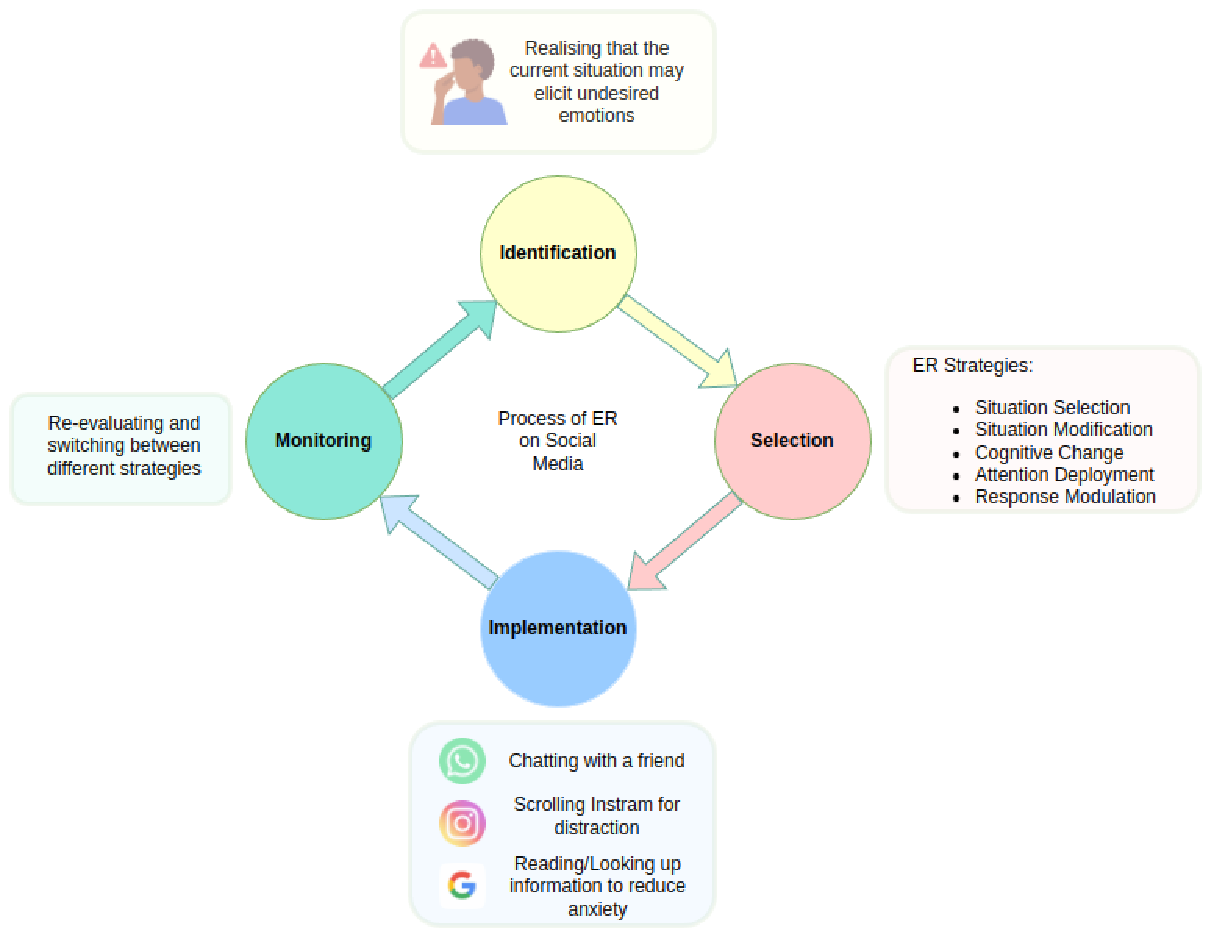
\includegraphics[width=14cm,height=14cm,keepaspectratio]{ERProcess.pdf}
  \caption{Process of Emotion Regulation}
  \label{fig:Process}
  \end{figure}
  
  
The examples discussed thus far in this article are cases of intrinsic ER, wherein individuals seek to alter their personal affective states, but, in digital technologies, extrinsic ER is an essential component, where people intentionally try to influence the emotional state of others. Social media platforms allow users to create identifiable profiles, represent public connections and consume, produce, and/or interact with a wide range of user-generated content from their connections on the site. These applications consistently harbour communication among millions of people from all over the world and hence contain traces of emotional expression in abundance. Since the virtual world offers an opportunity to network with people beyond geographical boundaries, exposure to the expressions of others amplifies. As a result, the emotions, actions and online behaviours of the users can be strongly influenced. Given that user engagement is a key factor in the success of social media platforms, and exposure to emotion increases it, social media companies have strategically used the emotional effects of activities on social media platforms to improve user experience and fuel user participation. This intervention by digital media companies to boost the intensity and frequency of expression has resulted into increased online emotion contagion, which is the spontaneous spread and convergence of emotion based on exposure \cite{goldenberg2020digital}. According to ER psychological research, emotion contagion can be caused by extrinsic emotion regulation \cite{elfenbein2014many}. Online movements such as \#MeToo and toilet paper hoarding during COVID-19 (\#panicbuying), which rely on users' connected behaviours and have an impact on users' offline lives as well, emerged as a result of emotional contagion. Implicit emotion regulation, which does not involve a conscious desire to alter emotional responses, may also play a role in the development of connective action \cite{mirbabaie2021development}. Nonetheless, this disproportionate induction and convergence of emotion, generates social dysfunction and online toxicity.


There is still a substantial difference between online and offline social behaviour, even though the boundary between the real and the virtual is dissolving as technology becomes an inevitable part of our life. Although online toxicity has been well understood, recognised, and intensively studied for a few years now, remedial measures are challenging to implement due to the nature of online media environments, where the context of user behaviours cannot always be extracted \cite{slovak2022designing}, \cite{tag2022emotion}, \cite{thomas2022s}. Anonymity in social media platforms keeps the users behind the safety of a keyboard. This lack of accountability in social media platforms has adversely impacted online well-being. What is acceptable online (due to lack of mediation, moderation, or other restrictions), may not be accepted offline. As a result, it is crucial to understand and encourage responsible use of digital technology to regulate emotions effectively.


\subsection{Aim \& Objectives}~\label{subsec:aims}

The main contributions of this proposed research are described below:
\begin{itemize} 
    \item A model for on-the-spot attention and response modulation support in online conversations by encouraging self-reflection in moments of ongoing highly elevated emotional expression. The proposed model employs a graph-based framework to identify the need for emotion regulation in online social media conversations by incorporating text-based emotion recognition and toxicity analysis to locate the presence of intensified emotional expression and unfair induction of negativity. By locating these nodes in the conversation graph, this model provides users with a synopsis of their emotional impact on the conversation as well as design implications for social media applications to incorporate support for users' emotional regulation.
    \item A new method for calculating the effect of an induced emotion on a conversation. According to research, negative or rage-inducing emotions spread faster than positive ones. We aim to propose a new strategy for computing the impact of various emotions present in a post/online activity/conversation using this method by empirically evaluating the effectiveness of treating unlike emotions differently.
    \item A new machine learning-based recommender system for context-based emotion regulation strategy recommendation. After identifying the need for emotional regulation in an online environment, it is essential to provide support for the effective regulation of emotions by suggesting adequate techniques for the same. The goal here is to minimise suppression of emotions (as it leads to emotion dysregulation in the long-term) but rather trigger self-reflection and implicit emotion regulation.

\end{itemize}

\subsection{Structure}~\label{subsec:structure}
The remainder of this article is organised as follows. Section~\ref{sec:literature} reviews the literature for Digital Emotion Regulation, along with the interventions for identifying Emotion Regulation in online environments. Section~\ref{sec:design} presents the proposed model for on-the-spot emotion regulation support in online conversations. Section~\ref{sec:approach} describes the method for calculating the effect of an induced emotion on a conversation. Section~\ref{sec:evaluation} elaborates on the machine learning-based recommender system for context-based emotion regulation strategy recommendation. Finally, Section~\ref{sec:discussion} discusses the future plan for this proposed research. 
